\documentclass[a4paper]{article}
\usepackage[brazilian]{babel}
\usepackage[utf8]{inputenc}
\usepackage{graphicx}
\usepackage{caption}
\usepackage{indentfirst}
\usepackage{float}
\usepackage{setspace}
\usepackage{fancyhdr}
\usepackage{amssymb}
\usepackage{amsmath}
\usepackage{amsfonts,amssymb}
\usepackage{hyperref}
\usepackage{color}
\usepackage{listings}
\usepackage[top=2cm,left=2.85cm,right=2.85cm,bottom=2.6cm]{geometry}
\newcommand{\HRule}{\rule{\linewidth}{0.5mm}}
\renewcommand{\baselinestretch}{1.2}
\setlength{\parskip}{0.5\baselineskip}
\captionsetup[figure]{labelfont={bf},name={Fig.},labelsep=period}
\usepackage{subfig}

\begin{document}
\vspace{6mm}
\begin{center}
\Huge\textbf{Columnar Cactus Identification}
\end{center}
\vspace{3mm}

\begin{figure}[H]
\centering

\includegraphics[width=8cm,height=8cm]{sysu.png}
\end{figure}

\begin{center}
\large\textbf{16340154 -- Nino Lau }\\
\vspace{2mm}
\large\textbf{16340143 -- Albert Sheldon }\\
\vspace{2mm}
\large\textbf{16340134 -- John Doe }\\
\end{center}

\begin{center}
\normalsize{School of Data and Computer Science, Sun Yat-sen University}
\end{center}

\begin{center}
\textit{April. $27^{nd}$ \textit, 2019\\}
\end{center}
\vspace{8mm}

\begin{figure}[H]
\centering
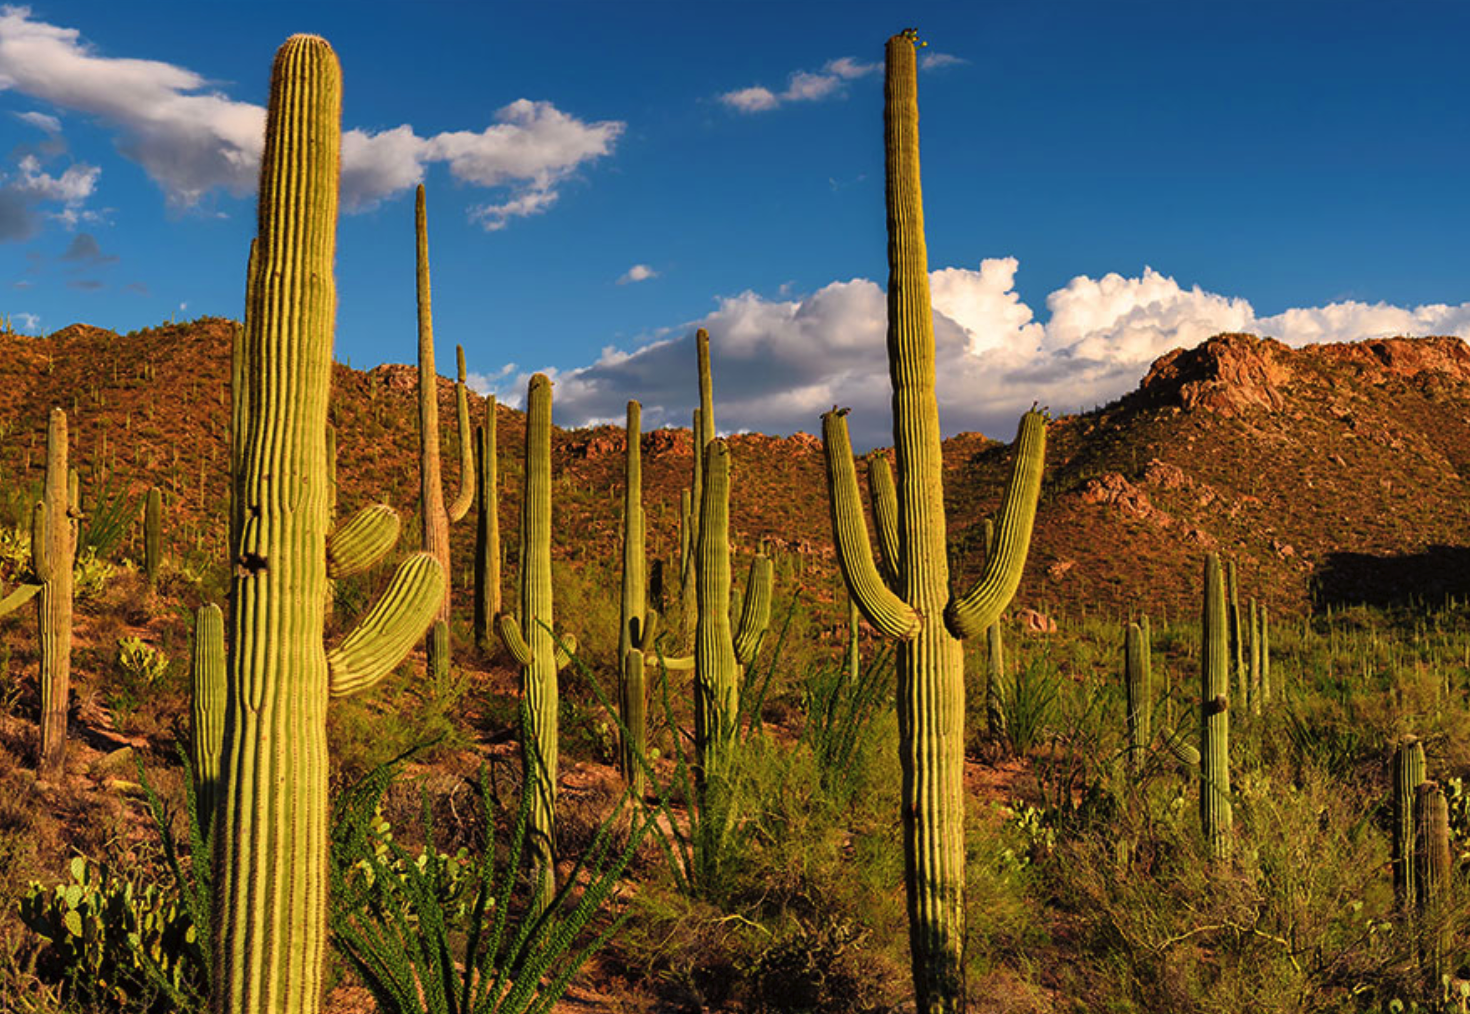
\includegraphics[width=15cm,height=9.8cm]{cactus.png}
\end{figure}

\noindent \HRule
\vspace{2.5mm} \\
\large{\textbf{Abstract. }\emph{In order to recognize the vegetation inside the protected areas, we are aiming to build models to identify a specific type of cactus from UAV. Five models (\textsf{VGG-Net, DenseNet, ResXNet ...}) are tried in \emph{Kaggle competition: Aerial Cactus Identification}. Experiment results shows that all models have great outcome, and ... model is the most accurate model among the five. In addition, some insights are proposed pinpointing the methods we used in this competition. \\ }}
\vspace{2mm}
\HRule

%%
\vspace{6mm}
\begin{center}
\LARGE\textbf{I. Introduction} \\
\end{center}
\vspace{2mm}

\large{\noindent To assess the impact of climate change on Earth's flora and fauna, it is vital to quantify how human activities such as logging, mining, and agriculture are impacting our protected natural areas. Researchers in Mexico have created the \href{https://jivg.org/research-projects/vigia/}{VIGIA project}, which aims to build a system for autonomous surveillance of protected areas. A first step in such an effort is the ability to recognize the vegetation inside the protected areas. We are tasked with creation of an algorithm that can identify a specific type of cactus in aerial imagery. 

Facing such challenge, we try 5 models to deal with the columnar cacti detection:

\begin{itemize}
    \item \textbf{VGG-Net}: \textsf{VGG-Net} is a deep convolutional neural network proposed by Visual Geometry Group. It's proved that \textsf{VGG-Net} has good results on the prior-art configurations and it also generalizes well to other datasets.
    \item \textbf{DenseNet}: 
    \item \textbf{ResXNet}: 
\end{itemize}

}



\clearpage

%%
\vspace{5mm}
\begin{center}
\LARGE\textbf{II. VGG Model} \\
\end{center}
\vspace{2mm}

\large{\underline{You can see our kernel submission page in \textbf{Appendix.} B.}}

\vspace{2mm}
\begin{center}
\large\textbf{Architecture} \\
\end{center}


\large{
In our first model, after trials and errors, we lock our target to a \textsf{VGG-16} model. 

\vspace{5mm}

\begin{figure}[H]
\centering
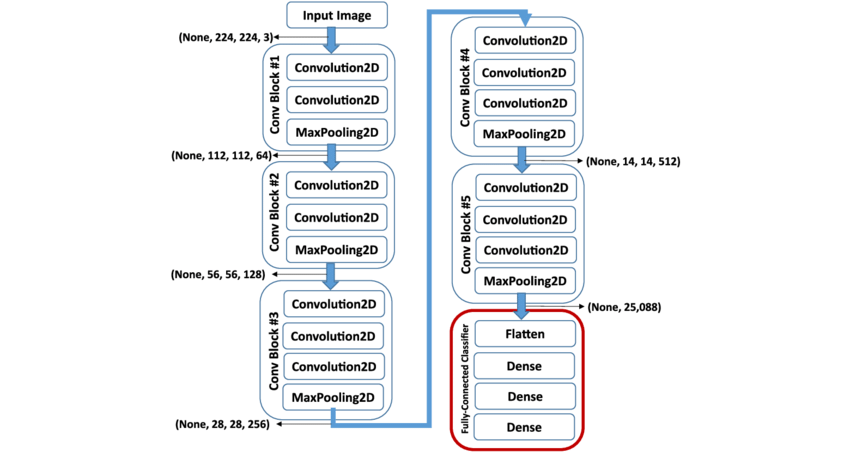
\includegraphics[width=16cm,height=9cm]{A-schematic-of-the-VGG-16-Deep-Convolutional-Neural-Network-DCNN-architecture-trained.png}
\caption{\textsf{VGG 16 Deep Convolutional Neural Network architecture.}}
\label{vgg16}
\end{figure}
\vspace{5mm}
Our network structure is very neat, and there are not so many super parameters. Focusing on the construction of a simple network, convolution layers are all followed by a pool layer which can compress the images. The framework of our \textsf{VGG-16} model is shown in \textbf{Fig. \ref{vgg16}.}

}

%%%%%
\vspace{2mm}
\begin{center}
\large\textbf{Implementation} \\
\end{center}

\large{

We first conduct data pre-processing operation, such as compose, pad, clip and normalization. Thus, the images in the dataset are rotated randomly and some bad examples are eliminated. Then the data is put into the network and the model is trained. We use \textsf{BCELoss} as our loss function and train the model for 40 times. Having tried many optimizing methods, \textsf{SGD} optimizer turns our to have relatively great performance as well as short converge time.

}

\large{\underline{You can see our model implementation in \textbf{Appendix.} C.}}
%%%%%
\vspace{2mm}
\begin{center}
\large\textbf{Results} \\
\end{center}

\large{

\textbf{Fig. \ref{vggresults}} shows the scatter plot of predicted values for 4000 samples and the histogram of predicted values for them.

}

\begin{figure}[H]
\centering
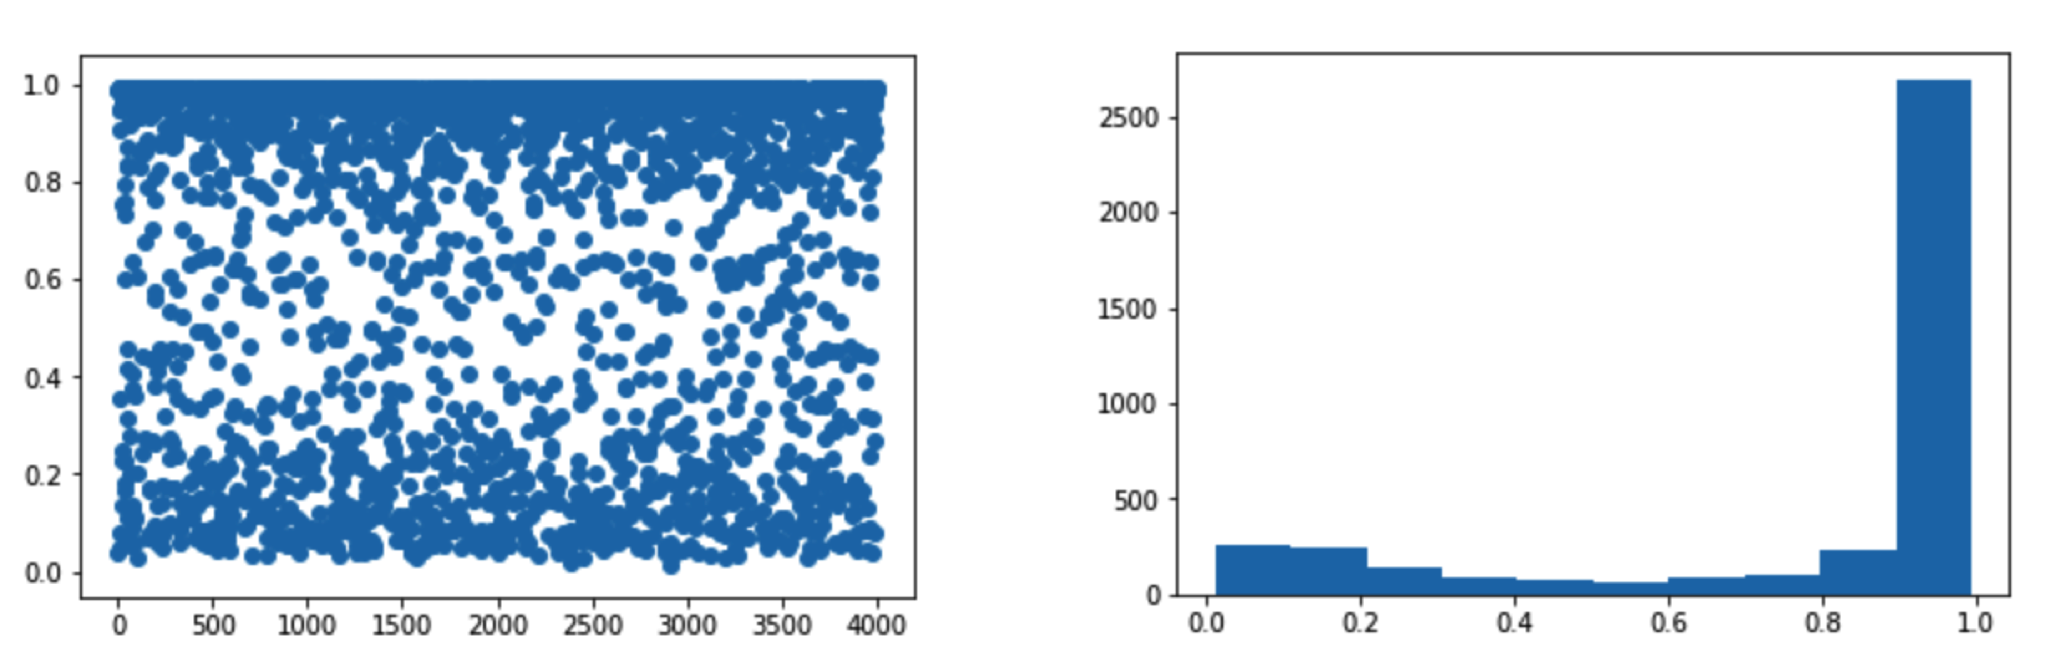
\includegraphics[width=15cm,height=6cm]{vggresults.png}
\caption{Prediction scatter and histogram.}
\label{vggresults}
\end{figure}

\large{
Our \textsf{VGG-16} model has an approximately 97\% accuracy on the training set, but seems to own defects on test set. So the final score is 0.5051 right now. We assume the probably shortcomings are out of main framework. We do not add additional transformed images in our dataset. Some other optimizer like Adam should also be taken into account. We will try these in our future work and explore some new methods.

}

%%
\vspace{15mm}
\begin{center}
\LARGE\textbf{IV. Conclusion} \\
\end{center}
\vspace{2mm}


%%
\vspace{1.5cm}
\begin{center}
\LARGE\textbf{V. Acknowledgement} \\
\end{center}
\vspace{.5mm}

\begin{itemize} \item{First and foremost, I would like to show my deepest gratitude to my teacher, professor \textbf{Roy Wang}, who has provided us with valuable theoretical guidance of deep learning. Without his enlightening instruction, impressive kindness and patience, I could never have completed our projects. His keen and vigorous academic observation enlightens me in this thesis and my future study.}
\item{My sincere appreciation also goes to our \textbf{teacher assistants}. We got along in harmony, accomplished tasks together, and they give me valuable advice. All of these make this experience meaningful.}
\end{itemize}

\clearpage
%%
\vspace{5mm}
\begin{center}
\LARGE\textbf{VI. Appendices} \\
\end{center}

\vspace{5mm}
\begin{center}
\large\textbf{A. Competition} \\
\end{center}

\large{
\begin{itemize}
    \item \textbf{Competition}: \underline{\href{https://www.kaggle.com/c/aerial-cactus-identification/overview}{Aerial Cactus Identification (\emph{Playground})}}
    \item \textbf{Time Line}: The competition will conclude July 8, 2019 at 11:59 PM UTC. 
    \item \textbf{Dataset}: $32 \times 32$ thumbnail columnar cactus images.
    \item \textbf{Target}: Creating a classifier to predict the probability of containing cactus.
\end{itemize}
}

\vspace{5mm}
\begin{center}
\large\textbf{B. Submission Pages} \\
\end{center}


\vspace{2mm}
\large{
Submission pages of our 5 models are listed as follows.
\begin{itemize}
    \item \textbf{VGG-16}: \underline{\href{https://www.kaggle.com/albertsheldon/kernel4651e4a6da}{https://www.kaggle.com/albertsheldon/kernel4651e4a6da}}
    \item \textbf{DenseNet}:
    \item \textbf{ResXNet}:
\end{itemize}
}

\vspace{5mm}
\begin{center}
\large\textbf{C. Implementation} \\
\end{center}

\vspace{5mm}

\noindent \normalsize \textbf{1) VGG-model.py} \small

\noindent \HRule

\lstinputlisting[language=python]{./VGGkernel.py}

\noindent \HRule

\vspace{1.5cm}

% \noindent \LARGE \textsc{2) utils.py} \small

% \noindent \HRule

% \lstinputlisting[language=python]{./utils.py}

% \noindent \HRule

% \vspace{1.5cm}

% \noindent \LARGE \textsc{3) datasets.py} \small

% \noindent \HRule

% \lstinputlisting[language=python]{./datasets.py} 

% \noindent \HRule

% \vspace{2cm}


\end{document}
